\begin{figure}[htbp]
\centering
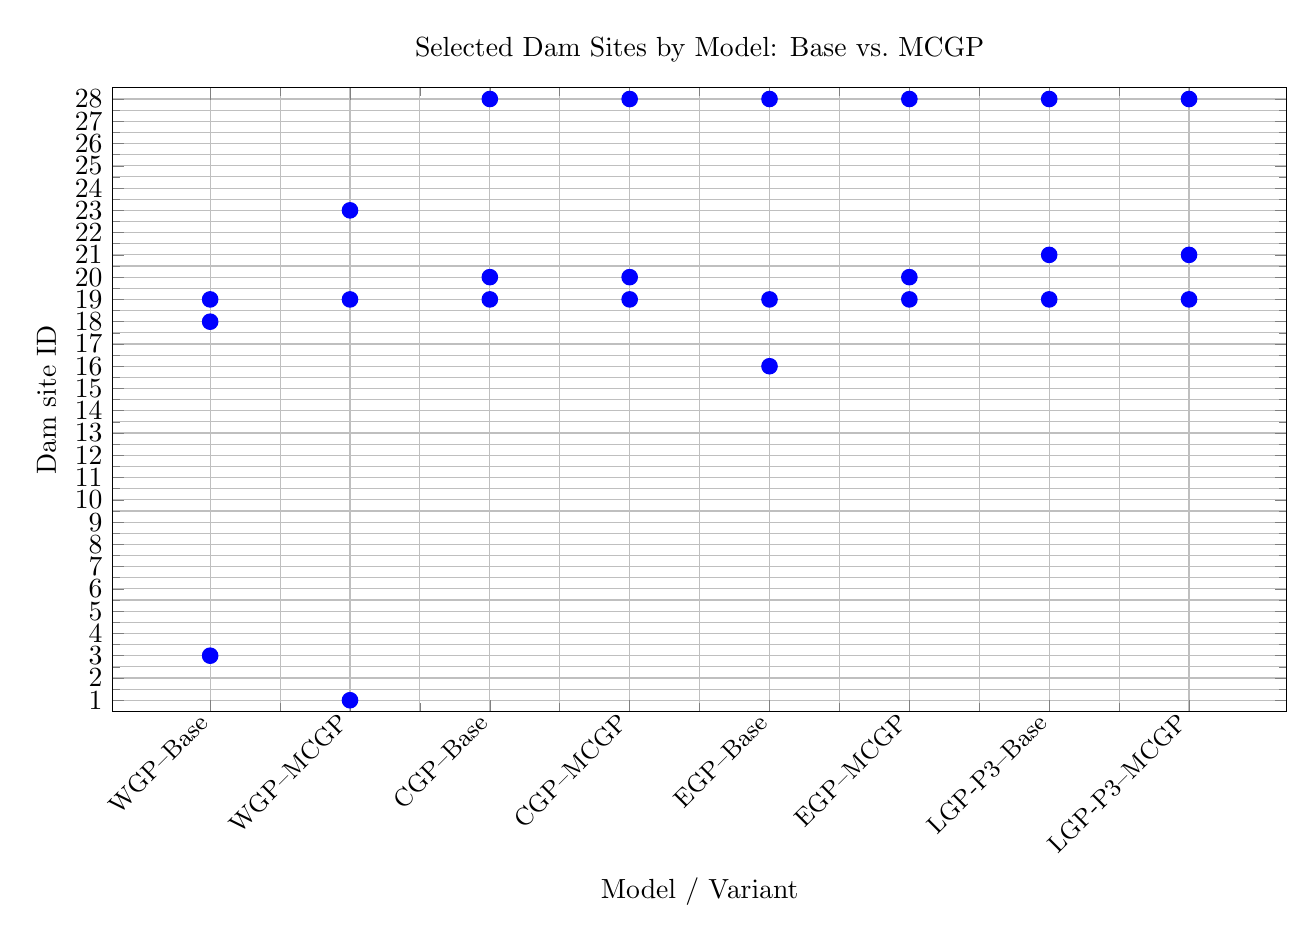
\begin{tikzpicture}
\begin{axis}[
  title={Selected Dam Sites by Model: Base vs.\ MCGP},
  xlabel={Model / Variant},
  ylabel={Dam site ID},
  symbolic x coords={
    WGP--Base,WGP--MCGP,
    CGP--Base,CGP--MCGP,
    EGP--Base,EGP--MCGP,
    LGP-P3--Base,LGP-P3--MCGP
  },
  xtick=data,
  ymin=0.5, ymax=28.5,
  ytick={1,2,...,28},
  x tick label style={rotate=45,anchor=east,font=\small},
  width=16.5cm, height=9.5cm,
  grid=both, minor tick num=1
]

% All points same color (blue circles)
\addplot+[only marks, mark=*, mark options={fill=blue, draw=blue}, mark size=2.8pt]
  coordinates {
    % ---------- WGP ----------
    (WGP--Base,3) (WGP--Base,18) (WGP--Base,19)
    (WGP--MCGP,1) (WGP--MCGP,19) (WGP--MCGP,23)

    % ---------- CGP ----------
    (CGP--Base,19) (CGP--Base,20) (CGP--Base,28)
    (CGP--MCGP,19) (CGP--MCGP,20) (CGP--MCGP,28)

    % ---------- EGP ----------
    (EGP--Base,16) (EGP--Base,19) (EGP--Base,28)
    (EGP--MCGP,19) (EGP--MCGP,20) (EGP--MCGP,28)

    % ---------- LGP-P3 ----------
    (LGP-P3--Base,19) (LGP-P3--Base,21) (LGP-P3--Base,28)
    (LGP-P3--MCGP,19) (LGP-P3--MCGP,21) (LGP-P3--MCGP,28)
  };

\end{axis}
\end{tikzpicture}
\caption{Selected dam sites for each model under Base and MCGP formulations. All markers are blue circles; x-axis labels indicate the model variant.}
\label{fig:site_selection_base_vs_mcgp}
\end{figure}
